\documentclass[14pt]{beamer}
%\documentclass[a4paper]{article}
%\usepackage[envcountsect]{beamerarticle}

\usepackage{color}
\usepackage{tikz}

\mode<presentation>
{
\usetheme{AlpesLasers}
\setbeamercovered{transparent}
  %\setbeamertemplate{footline}[frame number] 
  %\setbeamertemplate{navigation symbols}{ 
  %\hskip 0.3cm
  %\insertframenumber / \inserttotalframenumber  % <<< frame #
  %\insertpagenumber / \insertpresentationendpage % <<< page #
%} 
}

% font definitions, try \usepackage{ae} instead of the following
% three lines if you don't like this look
\usepackage{listings}
\lstloadlanguages{python}

\usepackage{mathptmx}
\usepackage[scaled=.90]{helvet}
\usepackage{courier}
\usepackage[T1]{fontenc}
\usepackage[english]{babel}
\usepackage[latin1]{inputenc}
\title{Designing an efficient simulation framework}
%\subtitle{A little overview}
\author{St\'ephane Poss}
\date{\today}
% This is only inserted into the PDF information catalog. Can be left
% out.

\lstdefinestyle{custompy}{
  belowcaptionskip=1\baselineskip,
  breaklines=true,
  xleftmargin=\parindent,
  language=python,
  showstringspaces=false,
  basicstyle=\footnotesize\ttfamily,
  keywordstyle=\bfseries\color{green!40!black},
  commentstyle=\itshape\color{purple!40!black},
  identifierstyle=\color{blue},
  stringstyle=\color{orange},
}
\lstdefinestyle{customsh}{
  belowcaptionskip=1\baselineskip,
  breaklines=true,
  xleftmargin=\parindent,
  language=bash,
  showstringspaces=false,
  basicstyle=\footnotesize\ttfamily,
  keywordstyle=\bfseries\color{green!40!black},
  commentstyle=\itshape\color{purple!40!black},
  identifierstyle=\color{blue},
  stringstyle=\color{orange},
}
\lstdefinestyle{customcpp}{
  belowcaptionskip=1\baselineskip,
  breaklines=true,
  xleftmargin=\parindent,
  language=C++,
  showstringspaces=false,
  basicstyle=\footnotesize\ttfamily,
  keywordstyle=\bfseries\color{green!40!black},
  commentstyle=\itshape\color{purple!40!black},
  identifierstyle=\color{blue},
  stringstyle=\color{orange},
}

\begin{document}
\begin{frame}[plain]
\titlepage
\end{frame}

\begin{frame}
\tableofcontents
\end{frame}

\section{Motivation}
\begin{frame}
\frametitle{Why this training?}

\includegraphics[width=\textwidth]{comp_prog_works_but_dangerous}
\end{frame}
\note{This training is designed to show you the issues faced by (mostly) students during their PhD when it comes to using computers to do part of the work. As the illustrations shows, it's a 'normal' situation. I do not know anybody that did not have this case at least once.}

\begin{frame}
\centering
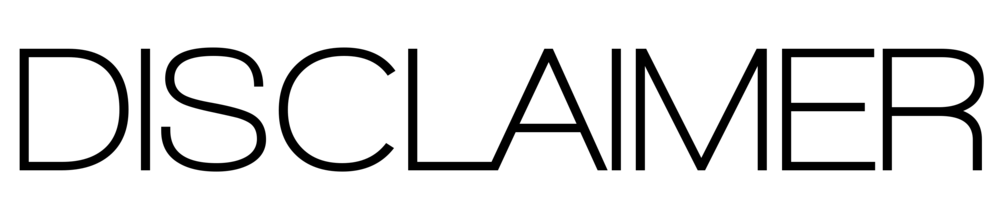
\includegraphics[width=0.7\textwidth]{disclaimer}

\end{frame}
\note{The following presentation is the results of years of troubles, 3 work places with different practices, and discussions with friends/colleagues. It may not represent the complete situation, and some of the topics mentioned here can be already known by some people. I tried to collect the worst practices and the best ideas to fix them, and I may have missed some things.}

\begin{frame}
Ch. Hugon, INFN fellow:
\begin{quote}
Maybe it's not worth telling people about this stuff, maybe it's worth for them to discover the do's and don'ts by themselves...
\end{quote}
\end{frame}
\note{This quote from a friend of mine, former colleague and student is representative of the current state of affairs: it's hard to teach this stuff, and showing things may not be enough, you'd need to experience them to feel the pain. Nevertheless, maybe this talk will give you tools to face the problems in a sane manner.}

\section{Definitions}
\begin{frame}

\includegraphics[width=\textwidth]{definition}
\end{frame}

\begin{frame}
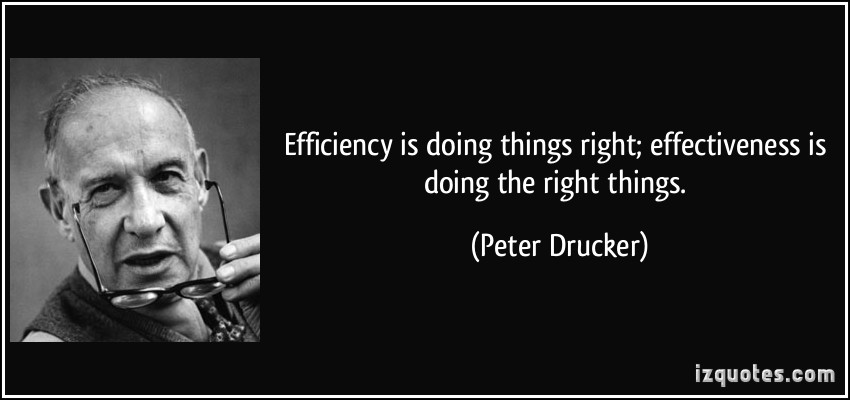
\includegraphics[width=\textwidth]{quote-efficiency-is-doing-things-right-effectiveness-is-doing-the-right-things-peter-drucker-53210}
\end{frame}
\note{Efficiency and effectiveness are complementary. I will concentrate on the first, as it's not my role to tell what you should do. I will tell you how though.}


\begin{frame}
\frametitle{Simulation framework}
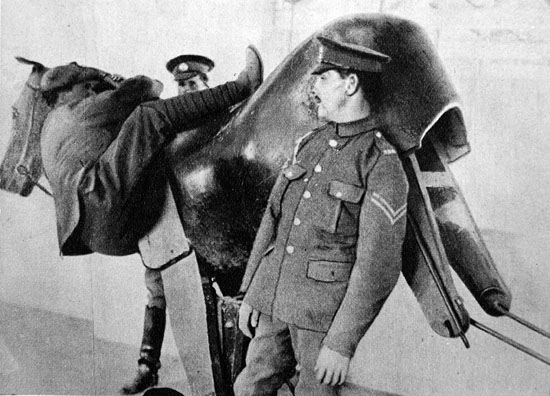
\includegraphics[width=\textwidth]{Horse_simulator_WWI}
\end{frame}
\note{Defining simulation framework goes to defining modeling. Wikipedia has a nice article on this, where the image is taken from. It's a horse simulator used during WW1. It's important to define properly what we mean by simulation as it drives the rest of the talk.}

\begin{frame}
\frametitle{Why simulations?}
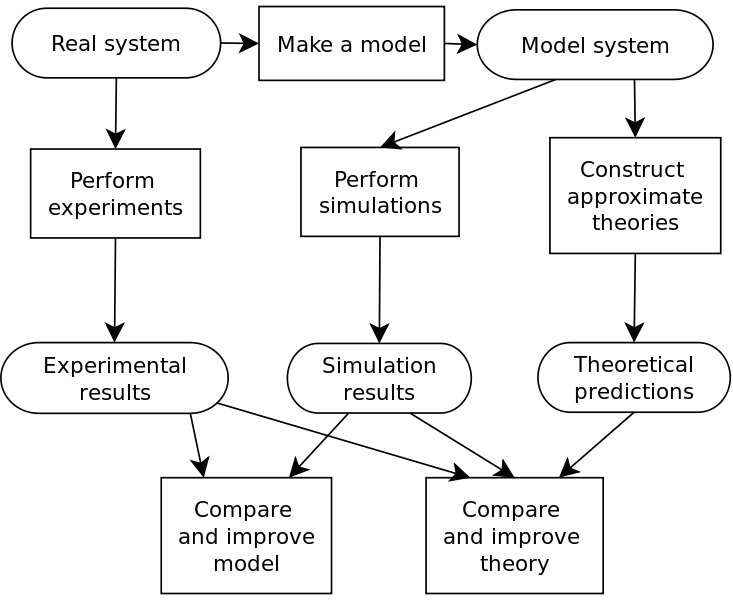
\includegraphics[width=\textwidth]{733px-Molecular_simulation_process}
\end{frame}
\note{Starting from a real life situation, we want to put a theory on it, because we want to predict the future behavior of the system. If there is a theory, there is a model. The model may not be a complete representation of the theory. Thus, the simulation has 2 purposes: improve the model when comparing with experiment, or improve the theory by numerically checking its soundness.}

%\begin{frame}
%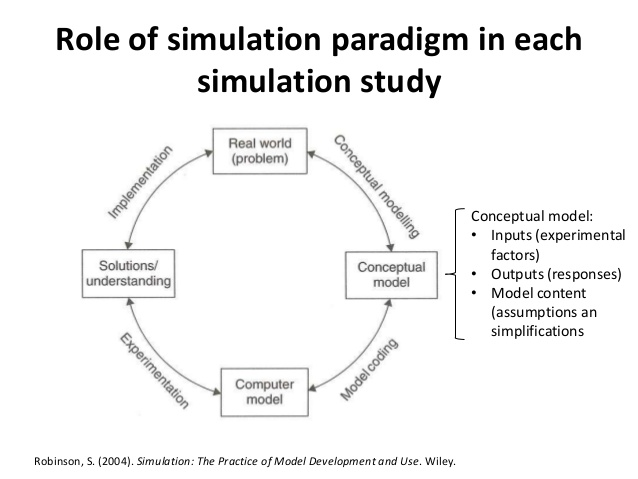
\includegraphics[width=1.1\textwidth]{agentbased-modeling-system-dynamics-or-discreteevent-simulation-modeling-paradigm-for-supply-chains-simulation-3-638}
%\end{frame}
%\note{This shows more or less the same ideas as previously}

\begin{frame}
\alert{Simulations are essential for science!}
\end{frame}


\section{The usual situation}
\begin{frame}
\frametitle{The usual situation}

\includegraphics[width=\textwidth]{painful_but_true}
\end{frame}
\note{I will now tell you a bit about how things are usually done during a PhD (and beyond). It's a bit ugly and some of you may laugh due to experience.}

\begin{frame}
\frametitle{1st year PhD}
\begin{itemize}
\item Create files on the fly, in the same directory
\item Overwrite code, changes drastically every day, DRY principle NOT applied
\item Output are named test\_1, test\_2, test\_1\_altered, lum\_check\_260815, plots are all in the same directory
\item Code monolithic as much as possible, data structure unclear
\end{itemize}
\end{frame}
\note{
A big mess! Usually, you don't have any idea about you are doing then, so you do not think ahead. Not your fault! So you tend to overwrite stuff, both files and code, without thinking that some results may have already been found. 

Also, in the code, you usually have one big file containing one big function, called main, which contains all the code you can think of. As for the handling of the inputs and outputs, there is no clear logic: it's done as it comes. Usually, you'd have many times the same main function, in different code pieces. The Don't Repeat Yourself principle is not applied at all!
}

\begin{frame}
\frametitle{1st year PhD}
\begin{itemize}
\item Application version does not matter, hacked to fit need if possible.
\item Data stored only on personal drive, not backed up
\item Sharing of code/data via email, but unusable
\item All analysis are slightly different, can hardly be shared between run points
\end{itemize}
\end{frame}
\note{In case you use an external application (commercial software is legion in this domain), you tend not to care too much about the version and the features: as long as it does what you want (or what you think you want), you are good to go. True? NO! Applications are buggy in general, or there is one corner case that isn't handled yet, and eventually, you need to change the version. As for data: it's stored usually on your own computer despite the availability of other solutions (not so true anymore due to google drive and such). What happens if computer dies? 

Sharing information with colleagues is funny too: you send them some code and some data files, they come back to you with a little problem, making you realize that to process the data, you'd have to look thru old code version, which you do not have due to the situation before! So you have to rewrite lots of code!

In any case, you'd have many version, slightly different, of essentially the same thing!
}

\begin{frame}
\frametitle{2nd year PhD}
\begin{itemize}
\item Use directory structure\\ /data/thesis/simu/260815/p1/p2/file\_p1\_p2.out, input.txt, source code
\item Code organized by date: changes imply copy of the code structure
\item Code structured: reused functions appear
\item Application version is checked regularly, new features asked to dev being added on demand (if possible)
\end{itemize}
\end{frame}
\note{Situation a bit better: you use a proper directory structure that holds some meta information about your data (more on that later), and your code is now organized by date: you have many copies, but they each have a date. Even better, the many versions of your code tend to re-use functions! 

You are now aware that your commercial application tends to evolve, possibly thanks to your input, so you now take that into account. 

Several questions remain:
\begin{itemize}
\item How to add info in fixed path? variable and rigid
\item How do you know which code contains which change?
\end{itemize}
}
\begin{frame}
\frametitle{2nd year PhD}
\begin{itemize}
\item Log book used
\item Data shared via NFS/FTP/SCP/etc. 
\item Recipes to process data in place, still done manually
\end{itemize}
\end{frame}
\note{
\begin{itemize}
\item logbook: more or less efficiently and effectively: link data and dates and inputs and outputs. Huge work to write those down, so sometimes you don't do it because everyone is lazy. 
\item data sharing: use transfer protocols, no mail
\item data processing: in the logbook. But no one else, plus code changes often still
\end{itemize}
}

\begin{frame}
\frametitle{3rd year PhD}
\begin{itemize}
\item Meta description of data
\item Files stored on persistent drive
\item Synergy with application developer
\item Core applications wrapped to read/store I/O directly in DB
\item Code properly documented, API well defined and stable
\end{itemize}
\end{frame}
\note{
Finally, good practices arrive!
\begin{itemize}
\item flexible, extensible, easy to find what you want
\item Use relational databases
\item setup backup procedures: backup, distributed, shared
\item Interactions between data storage and processing simplified
\end{itemize}
}

\begin{frame}
\frametitle{3rd year PhD}
\begin{itemize}
\item Code structured properly
\item Code versioning used extensively
\item Automatic processing of data
\item Use code from elsewhere
\end{itemize}
\end{frame}
\note{
\begin{itemize}
\item Code is organized in logical elements, core libraries stand out and reused. data structures are decoupled from functions
\item SVN/GIT
\item workflows, data driven processing
\item Don't reinvent the wheel
\end{itemize}
}

\section{Where we go from there}
\begin{frame}
\centering
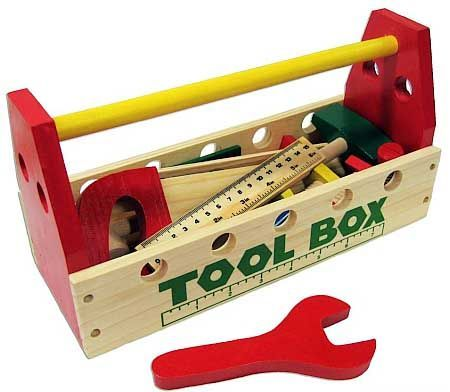
\includegraphics[width=0.8\textwidth]{wooden_tool_box}

\end{frame}
\note{Following slides show the tools that are useful}

\subsection{Coding practices}
\begin{frame}
\frametitle{Version control}
\centering
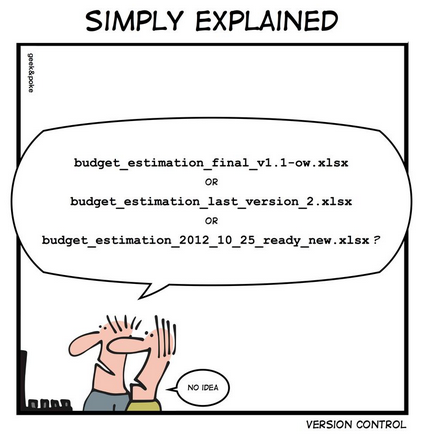
\includegraphics[width=0.8\textwidth]{Version-Control-Comic}

\end{frame}

\begin{frame}
\frametitle{Version control}
\begin{block}{How?}
\begin{itemize}
\item[SVN] Centralized: need to get all changes from master server every time
\item[\alert{Git}] Distributed: all history local, can have many parallel copies
\end{itemize}

\includegraphics[width=0.5\textwidth]{svn-name-banner.jpg}$\quad$

\includegraphics[width=0.3\textwidth]{Git-Logo-2Color.png}
\end{block}
\end{frame}
\note{Version control is technically managed using essentially 2 tools: centralized version control and distributed version control. Shown here are 1 example of each. SVN is more traditional and is being phased out in favor of the latter. There are other distributed version control system with slightly different purposes, such as Bazaar or mercurial. I leave as an exercise to the student to look into them. Version contol will save your life if used properly.}

\begin{frame}
\frametitle{Version control utilities}
\begin{itemize}
\item Github
\item Gitlab
\item git-book\\ \url{http://www.git-scm.com/book/en/v2}
\end{itemize}
\end{frame}
\note{There are many ways of using git collaboratively. The most famous one is github. Another one, more recent and a bit more powerful is gitlab. Fianlly I can only recommend looking at the git-book, free and online}

\begin{frame}
\frametitle{Documentation}
\centering

\includegraphics[width=\textwidth]{docu}

\end{frame}
\note{
Documentation is fundamental! People tend to overlook it, because they don't see the point. They don't see that maybe, someday, someone will reuse their stuff. Or they think that no one cares. It's wrong!
}



\begin{frame}
\frametitle{Documentation}
\begin{itemize}
\item Code documentation isn't enough
\item Tests (if any) aren't enough
\item Think documentation as teaching
\end{itemize}
\url{http://docs.writethedocs.org/}\\
\url{http://sphinx-doc.org/}
\end{frame}
\note{ 
Remember there is someone that will be using your stuff after you left!

Tests should exist!
}

\begin{frame}
\frametitle{Documentation}
\centering
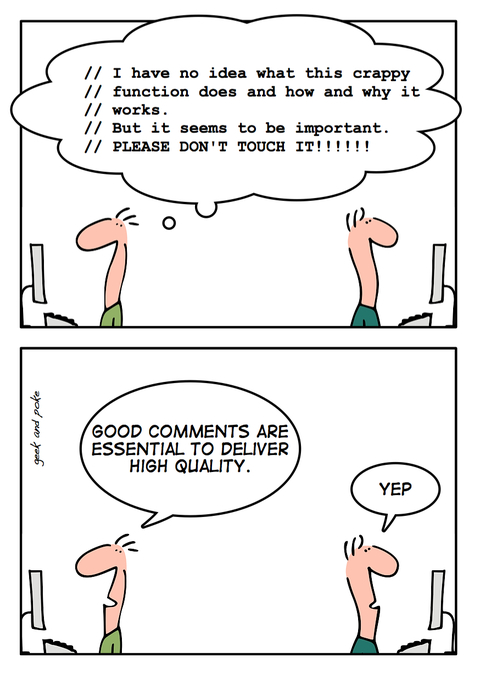
\includegraphics[width=0.6\textwidth]{goodcomments}

\end{frame}
\note{Example of bad doc!}

\begin{frame}
\frametitle{Coding practices}
\centering

\includegraphics[width=\textwidth]{dontrepeatyourself_motivator_2}

\end{frame}
\note{One of the core coding principles, often overlooked by beginners. You cannot imagine the risk and the time lost when you do not apply it. Clearly, an example of such practice is the development of an analysis tool chain where algorithms are to be used in several contexts e.g. finding the mean of a distribution.}

\subsection{PYTHON}
\begin{frame}

\includegraphics[width=\textwidth]{python-logo-master-v3-TM}\\
Perfect scripting language for the physicist!
\end{frame}
\note{Been using Python for many years. Prefer it to C++. Easy to learn and use. Lack of compilation saves many headaches.}

\begin{frame}
\frametitle{Python}
\begin{itemize}
\item C/C++: effective language, not efficient in its use, but efficient in CPU usage\\~
\item Python: effective and efficient language for the physicist, not as efficient in CPU cycles
\end{itemize}
\end{frame}
\note{Use the right language for a given purpose!}

\begin{frame}
\frametitle{Must-use libraries}
\begin{itemize}
\item numpy: matlab like interface to data
\item scipy: machine learning tools
\item pandas: data analysis
\item sympy: symbolic computations
\item matplotlib: plots
\item sqlalchemy: DB overlay
\end{itemize}
Many other utilities available!
\end{frame}
\note{There are 1000s of libraries free to use, but the most notable for the physics are here. Brief description of each.}

\begin{frame}
\centering

\includegraphics[width=0.5\textwidth]{PyCharm_Logo}\\
\url{http://www.jetbrains.com/pycharm/}
\end{frame}
\note{Present pycharm quickly, in a few words}


\begin{frame}
\centering
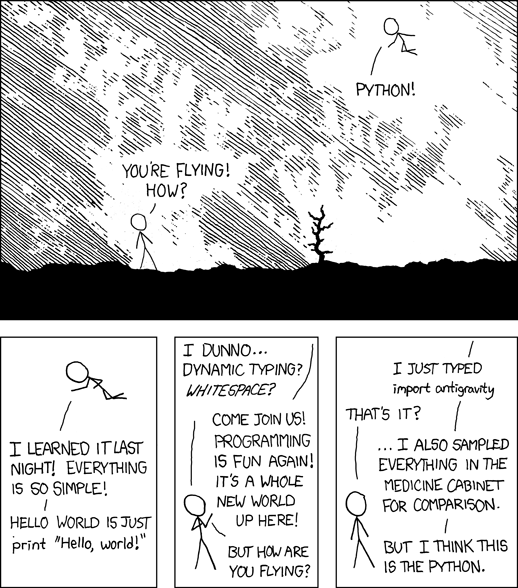
\includegraphics[width=0.7\textwidth]{python}

\end{frame}
\note{First time users of Python can be amazed by the language, and they get to do things very quickly! Much faster than with C++ or Java}

\subsection{Application control}
\begin{frame}
\frametitle{Control your applications}
\begin{itemize}
\item Control: keep track of your inputs and outputs
\item Know your application status
\item Ideally: connect your application with data I/O
\end{itemize}
\end{frame}
\note{Now moving on to the more conceptual things. In particular, the execution of an application, whichever it is. The first point I want to make is that it's of course essential to keep track of the I/O during a sequence of runs. Science is about reproducibility, and loosing track of something isn't scientific. The second point is that you should track your application status: failed/successful, and why. This is a needed info for 2 reasons: avoid rerunning failing things, and scanning your phase space for singularities, which can be very interesting as physical quantities. Finally, you want to be able to connect directly your application to your data storage, both input and output. Data storage means database in principle, but more on that now}

\subsection{Data storage}
\begin{frame}
\frametitle{Data storage and metadata}
Know your data: what, where?
\begin{itemize}
\item How to store data files?
\item Prefered: distributed, backed-up, DB backed system
\end{itemize}
Metadata:
\begin{itemize}
\item data about data or information about information
\end{itemize}
Technical solution?
\end{frame}
\note{When running a simulation, you need to know what you are doing (effectiveness). This imlies knowing your inputs and outputs, what they are, how they are represented. An input can be a number, a text file, a structure in a database, etc. I'll concentrate on the most classical way, using files as I/O. Managing those can be tricky, and I recommend using distributed systems, backed-up, with, if possible, a database backend for metadata. Metadata is the information about information. It is for example the temperature used during a simulation, or the structure ID. The date at which the file is present is also a useful meta information, so is the file size. They represent different types of metadata. There is in the litterature a large discussion on this topic, and I invite you to look for it. Assuming you go for the full thing, which you should, you'll need a means to control that metadata.}

\begin{frame}
\frametitle{Database systems}
RDBMS: SQL
\begin{itemize}
\item MySQL
\item PostgreSQL
\item Oracle
\end{itemize}
NoSQL
\begin{itemize}
\item MongoDB
\item CouchDB
\item Graph DB (ex. neo4j)
\end{itemize}
Python bindings available for most!
\end{frame}
\note{There are plenty of solutions for managing data using a database. Some are based on relational database systems, the SQL types, and there are more rencetly new types of DBs that appeared, the Not Only SQL DBs. The main difference is that the relational have at their core a relationship between items, while in the later it's more individual items, witout relationships. GraphDBs are particualr in the sense that they aren't table driven like a SQL solution, but graph driven, where every element is a node related to others via edges. I'm not too familiar with this, but it seems to me like the best idea to manage unpredictabe data. It's highly scalable and evolutive. All those solutions have in common the existence of python bindings, open source and free to use, making them easier to integrate with the rest.}


\begin{frame}
\frametitle{iRods}
Integrated Rule-Oriented Data System
\begin{itemize}
\item data discovery using a metadata catalog
\item automates data workflows
\item enables secure collaboration
\item implements data virtualization
\end{itemize}
\url{https://irods.org}
\end{frame}
\note{Advanced topic, only treated if enough time. iRods is a new complete solution that is being used in a few astrophysics communities. Allows storing petabytes of images and easily query them. The rule system allows automatic processing of data, although the rule language is rather cumbersome.}

\begin{frame}
\frametitle{Sumatra}
Track down your simulation provenance and results!\\
\url{neuralensemble.org/sumatra/}
\end{frame}
\note{This last project before going to the real life example is in a sense the complete solution to more or less everything I was ranting about before. This is a python project aimed at providing a tool to manage the simulations and the I/O. Simulations can be anything. If python, even better, but can be anything. Provides a DB to store code versions and the run result, has a web frontend for quick access, integrates with \LaTeX\ to include the plots with provenance information.

Moving on to the real life example.}

\section{Real life example}
\begin{frame}
\frametitle{Alpes Lasers simulation framework}
Goal:
\begin{itemize}
\item Simulate (predict) 1000s of QCL designs
\end{itemize}
~\\Problems:
\begin{itemize}
\item No on-site computing resources
\item $\approx70$ parameters
\item Fast runs: 2-3 minutes
\item Reduce costs
\end{itemize}
\end{frame}
\note{We want to simulate many different designs and study their properties. We are client driven so the costs must be under control. We have no on-site resources, so we need to use something cheap and available on demand. The simulations are are complex as they require 70 parameters or so, and they are fast, putting constrains on the data storage engine, more on that later.}


\begin{frame}
\frametitle{Alpes Lasers simulation framework}
Solutions:
\begin{itemize}
\item Cloud: AWS
\item Database
\item Python
\item Decouple application from task definition
\item Decouple task management from execution backend
\end{itemize}
\end{frame}
\note{We use AWS as a solution for computing. It's cheap, quick to start, alays available. interfaces well with python. I implemented a database to store the runs, more on that later. We traditionaly use Python in Alpes, and it's a great language for this. I decided to implenent a system where the execution of the application was decoupled from the task definition, making this asynchronous. It has the advantage that the task execution is then decoupled from the execution backend, i.e. if the chosen technical solution does not work, it's easy to change it.}

\begin{frame}
\frametitle{Alpes Lasers simulation framework}
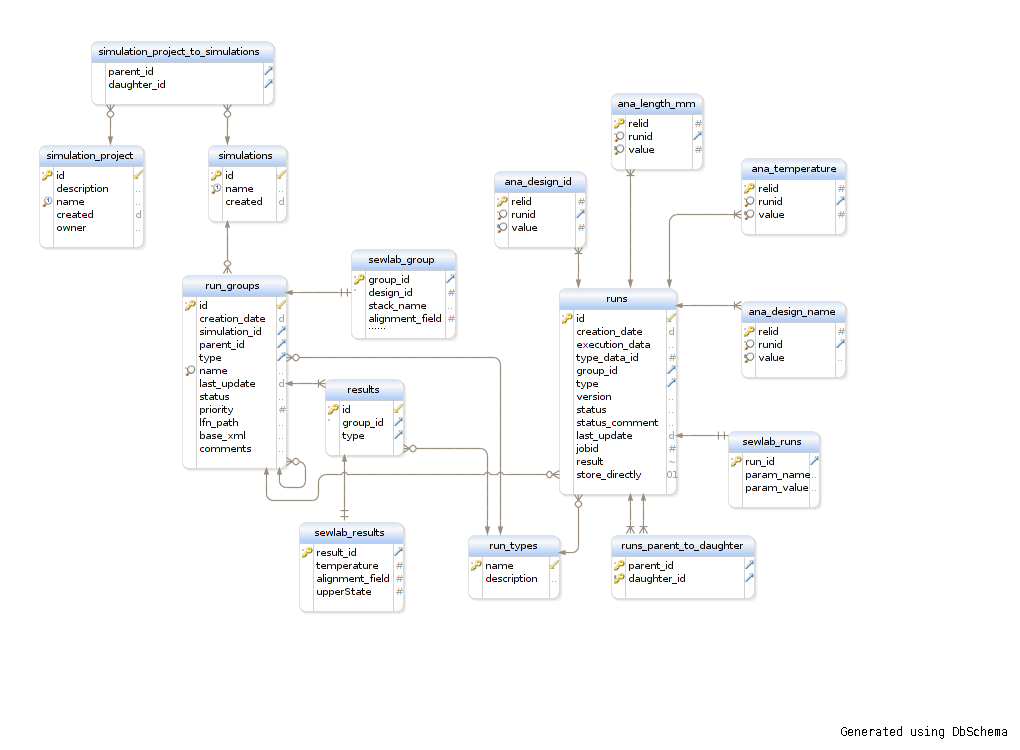
\includegraphics[width=1.3\textwidth]{simudb}
\end{frame}
\note{This shows the view of the simulation database I designed. All elements are described orally.}

\begin{frame}
\frametitle{Alpes Lasers simulation framework}
\lstinputlisting[language=python, style=custompy]{input.py}
\end{frame}
\note{As we use python, I show here an excerpt of the code needed to define a run. What is missing here are the definitions of the source objects and the DB connection. Those are technical details that users should never have to care about. In a later version, I hope to get rid of it. The important thing is that every step is properly defined, and the information stored in the DB. Every run has its set of meta information.}

\begin{frame}
\frametitle{Alpes Lasers simulation framework}
Tasks are executed by DIRAC\\
~\\
DIRAC is a complete distributed computing solution from CERN\\
~\\
Coupling lose: can be any backend that can read from DB.
\end{frame}
\note{For the task (or run) execution, we use a soluton I was using and partly developed when I was at CERN. It's a complete distributed computing solution called DIRAC (acronym irrelevant, just for the pun). As I said earlier, the system is designed so that where the tasks are defined is not related to DIRAC, it only reads/writes what is needed.}


\begin{frame}
\frametitle{Alpes Lasers simulation framework}
Finding data:
\lstinputlisting[language=python, style=custompy]{read.py}
\end{frame}
\note{Accessing information from the database can be done using this example code. The tricky bit here is the query syntax, but I used bits of code from DIRAC, modified (thus not copied) to fit my needs. 

Detail of the code.}


\begin{frame}
\frametitle{Alpes Lasers simulation framework}
System operational, used by many in the company
\end{frame}
\note{The current state of this is that it's being used for more than 1 application, which I cannot really talk about, by several people in the company to run their simulations. It seems to fit the needs as I did not need to touch it for more than a year!}

\section{Conclusions}
\begin{frame}
\frametitle{Conclusions}
\begin{itemize}
\item Many ideas
\item Many tools
\item Sometimes hard to implement
\item \alert{Really worth it!}
\end{itemize}
\end{frame}
\note{There are many ideas to improve your simulation frameworks, possibly some that I missed. There are many tools that can help in this task, and I hope I managed to give you the wish to look into some of those in a bit more detail. You should know that it's somtimes hard to use or to get your head around the ideas, but they are surely very much worth it.}
\begin{frame}
\centering

\includegraphics[width=0.7\textwidth]{doit}

\end{frame}
\note{In any case, you can certainly keep this in mind!}
\begin{frame}

\includegraphics[width=\textwidth]{sad_truth}
\end{frame}
\note{Finally, this is a rather sad truth, but the center boxes are the entire point I wanted to make here, I hope to have given you at least some ideas on how to deal with this stuff in the future, and teach your own students that some solutions exist.}
\end{document}
